\section{The SIR Model}
To explain the concepts of ABS and of our functional reactive approach to it, we introduce the SIR model as a motivating example. The SIR model is a a very well studied and understood compartment model from epidemiology which allows to simulate the dynamics of an infectious disease spreading through a population. In this model, people in a population of size $N$ can be in either one of three states \textit{Susceptible}, \textit{Infected} or \textit{Recovered} at a particular time, where it is assumed that initially there is at least one infected person in the population. People interact with each other \textit{on average} with a given rate $\beta$ per time-unit and get infected with a given probability $\gamma$ when interacting with an infected person. When infected, a person recovers \textit{on average} after $\delta$ time-units and is then immune to further infections. An infected person interaction with another infected one is never re-infected, thus interactions amongst infected people is not important in this model. This definition gives rise to three compartments with the transitions as seen in Figure \ref{fig:sir_transitions}.

\begin{figure}
	\centering
	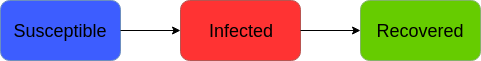
\includegraphics[width=.4\textwidth, angle=0]{./fig/SIR_transitions.png}
	\caption{Transitions in the SIR compartment model.}
	\label{fig:sir_transitions}
\end{figure}

The dynamics of this model over time can be formalized using the following equations:

$\frac{\mathrm d S}{\mathrm d t} = -infectionRate$ \\
$\frac{\mathrm d I}{\mathrm d t} = infectionRate - recoveryRate$ \\
$\frac{\mathrm d R}{\mathrm d t} = recoveryRate$ \\

$infectionRate = \frac{I \beta S \gamma}{N}$ \\
$recoveryRate = \frac{I}{\delta}$ \\

Solving these can be done using the System-Dynamics (SD) approach which solves the equations by integrating over time. In the SD terminology, the intergrals are called \textit{Stocks} and the values over which is integrated over time are called \textit{Flows}.

$S(t) = N + \int_0^t -infectionRate\, \mathrm{d}t$ \\
$I(t) = 1 + \int_0^t infectionRate - recoveryRate\, \mathrm{d}t$ \\
$R(t) = \int_0^t recoveryRate\, \mathrm{d}t$ \\

There exist a huge number of software-packages which allow to conveniently express SD models using a visual approach like in Figure \ref{fig:sir_sd_stockflow_diagramm}.

\begin{figure}
	\centering
	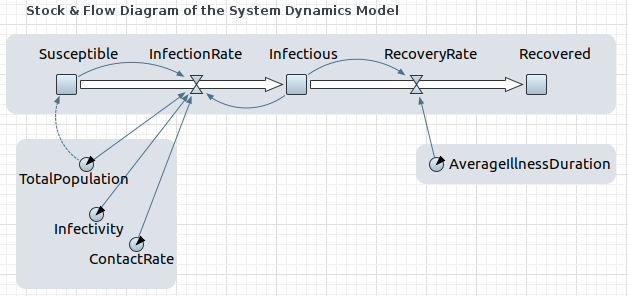
\includegraphics[width=.4\textwidth, angle=0]{./fig/SIR_SD_STOCKFLOW_DIAGRAMM.png}
	\caption{A visual representation of the stocks and flows in the SIR compartment model (Image courtesy of AnyLogic Company).}
	\label{fig:sir_sd_stockflow_diagramm}
\end{figure}

Running the SD simulation over time results in the dynamics as shown in Figure \ref{fig:sir_sd_dynamics_anylogic} with the given variables.

\begin{figure}
	\centering
	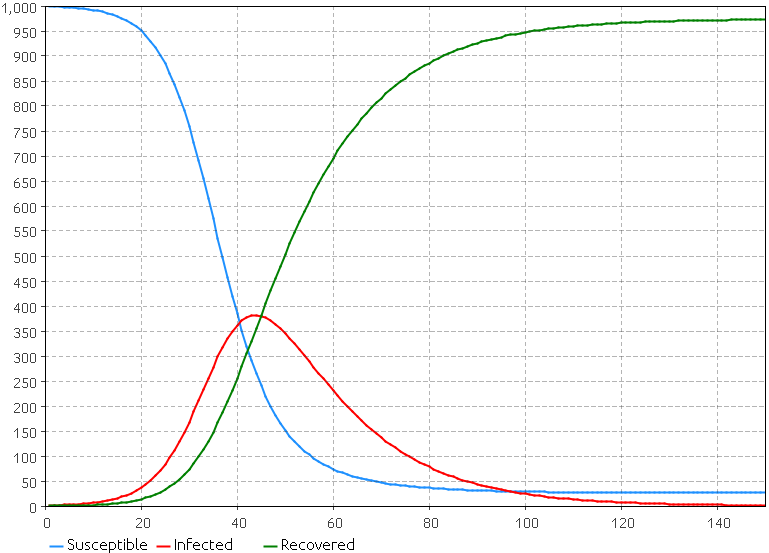
\includegraphics[width=.4\textwidth, angle=0]{./fig/SIR_SD_DYNAMICS_ANYLOGIC.png}
	\caption{Dynamics of the SIR compartment model using the System Dynamics approach generated with the AnyLogic Personal Learning Edition 8.1.0. Population Size $N$ = 1000, contact rate $\beta = 1/5$, infection probability $\gamma = 0.05$, illness duration $\delta = 15$.}
	\label{fig:sir_sd_dynamics_anylogic}
\end{figure}

\subsection{An Agent-Based approach}
The SD approach is inherently Top-Down because the emergent property of the system is formalized in differential equations. The question is if such a top-down behaviour can be emulated using ABS, which is inherently bottom-up. Also the question is if there are fundamental drawbacks and benefits when doing so using ABS. Indeed such questions were asked before and modelling the SD approach of the SIR model is possible using an agent-based approach. It is important to note that SD treats the population completely continuous which results in non-discrete values of stocks e.g. 3.1415 infected persons. Thus the fundamental approach to map the SIR model to an ABS is to discretisize the population and model each person in the population as an invidivual agent. The transition  between the states are no longer happening according to continuous differential equations but due to discrete events caused both by interactions amongst the agents and time-outs. The behaviour can be defined as follows:

\begin{itemize}
	\item Every agent makes on average contact with $\beta$ random other agents per time unit. In ABS we can only contact discrete agents thus we model this by generating a random event on average every $\beta$ time units.
	
	\item An agent does not know the other agents state when making contact with it, thus we need a mechanism in which agents reveal their state in which they are in \textit{at the moment of making contact}. Obviously the already mentioned messaging-mechanism which allows agents to interact is perfectly suited to do this.
	\begin{itemize}
		\item \textit{Susceptible} agent: sends a "Susceptible" message when contacting another agent. There is no need to reply to other incoming messages as making contact with a susceptible agent has no influence on the state of an agent.
		\item \textit{Infected} agent: sends a "Infected" message when contacting another agent. An infected agent now needs to reply to incoming "Susceptible" messages with an "Infected" message to let the susceptible agent know that it has made contact with an infected agent.
		\item \textit{Recovered} agent: does not need to send messages because contacting it or being contacted by it has no influence on the state.
	\end{itemize}
	
	\item Susceptible to Infected: needs to have made contact with an infected agent which happens when it receives an "Infected" message. If this occurs an infection occurs with a probability of $\gamma$. The infection can be calculated by drawing from a uniform random-distribution between 0 and 1 and comparing the value to $\gamma$, if the drawn value $p < \gamma$ then infection occurs. Note that this needs to be done for \textit{every} received "Infected" message.
	
	\item Infected to Recovered: a person recovers \textit{on average} after $\delta$ time unites. This is implemented by drawing the duration from an exponential distribution (TODO: borchschev) with $\lambda = \frac{1}{\delta}$ and making the transition after this duration.
\end{itemize}

We will discuss the implementation of this approach in the following sections and as will be shown FrABS will allow us to express this behaviour very explicitly looking very much like a formal ABS specification of the problem. For now we will give the resulting dynamics in Figure TODO

TODO: how many initially infected agents? one should be enough, at least in my implementation it is

TODO: 100 vs. 1000 vs. 5.000 agents

TODO: problem in my code: need exponentially occasionally not uniform distributed!
TODO: what differences do the different update strategies make?

\subsection{Blub}
TODO: It should be possible to formally show that spatial SIR and WildFire are the same model. NOTE: they are NOT the same, the fundamental difference is that in the WildFire model only the burning cells initiate the ignition - if we compare this to the SIR, the burning cells would be infected agents and although in the spatial SIR model the infected agents make contact with other agents, so do the susceptible ones which does NOT occur in wildfire

TODO: cite my own work on update-strategies

TODO: can we formally show that the SIR approximates the SD model?

TODO: cite papers which discuss how to approximate a SD model by ABS
- Macal (2010) - To Agent-Based Simulation From System Dynamics 
	-> i am very unhappy with this paper: first it does not give concrete parameters for the SD model so it is impossible to replicate. Also i think it has a systematical error as the infected agents make no contact but this is required as evident from the SD-models infection-rate which also incorporates. TODO: write an email to this guy: why are the infectious not contacting the other agents? this seems to be a systematical error
- Borshchev, Filippov (2004) - From System Dynamics and Discrete Event to Practical Agent Based Modeling: Reasons, Techniques, Tools
	-> its VERY IMPORTANT point is that we need to draw the illness-duration from an exponential-distribution because the illness-duration is proportional to the size of the infected. note: this is wrongly expressed, need to find the correct formulation

		-> my emulation of SD using ABS is really an implementation of the SD model and follows it - they are equivalent
		-> my ABS implementation is the same as / equivalent to the SD emulation
			=> thus if i can show that my SD emulation is equlas to the SD model
			=> AND that the ABS implementation is the same as the SD emulation
			=> THEN the ABS implementation is an SD implementation, and we have shown this in code for the first time in ABS
			
